\documentclass[12pt]{article}
\usepackage[utf8]{inputenc}
\usepackage[T1]{fontenc}
\usepackage{lmodern}
\usepackage{graphicx} % Required for inserting images
\usepackage{amsmath}
\usepackage{amsthm}
\usepackage{amsfonts}
\usepackage[english]{babel}



\usepackage[style=alphabetic,backend=biber,giveninits=true]{biblatex}
\addbibresource{bibliography.bib}
\usepackage[nottoc]{tocbibind}


\usepackage{etoolbox} 

\usepackage{epigraph}


\usepackage[shortlabels]{enumitem}
\usepackage{pstricks-add}
\usepackage{tikz}
\usetikzlibrary{decorations.pathreplacing}
\usetikzlibrary{patterns} % Pour les styles de traits
\usepackage[framemethod=TikZ]{mdframed}
\usepackage{tocloft}
\usepackage{hyperref}
\usepackage{amssymb}
\usepackage{ mathrsfs }
\usepackage{tikz-cd}
\usepackage{ stmaryrd }
\usepackage{cancel}
\usepackage{enumitem}
\usetikzlibrary{patterns,patterns.meta}
\usepackage[most]{tcolorbox}
\usepackage{titlesec}
\usepackage[normalem]{ulem}
\usepackage{comment}
\usepackage{microtype}
\usepackage{needspace}
\usepackage{xcolor}
\usepackage{mdframed}







\textwidth=18cm
\textheight=24cm
\oddsidemargin = -1truecm
\topmargin =-2truecm
\headsep =1truecm
\reversemarginpar
\marginparsep = -2cm
\parindent = 0truecm

%\usepackage{psfrag}
%\usepackage{graphicx}

%\usepackage{epsfig}

\tolerance=1000
\emergencystretch=1em



\pagestyle{plain}
\newcommand{\abs}[1]{ \left| #1 \right|}
\newcommand{\RR}{\mathbb{R}}
\newcommand{\NN}{\mathbb{N}}
\newcommand{\CC}{\mathbb{C}}
\newcommand{\ZZ}{\mathbb{Z}}
\newcommand{\QQ}{\mathbb{Q}}
\newcommand{\KK}{\mathbb{K}}
\newcommand{\LL}{\mathbb{L}}
\newcommand{\rg}{\text{rg}}
\newcommand{\Gal}{\text{Gal}}
\newcommand{\Vect}{\text{Vect}}
\newcommand{\diam}{\text{diam}}
\newcommand{\QQb}{\overline{\mathbb{Q}}}
\newcommand{\R}{\textbf{R}}
\newcommand{\N}{\textbf{N}}
%\newcommand{\CC}{\textbf{C}}
\newcommand{\Z}{\textbf{Z}}
\newcommand{\Q}{\textbf{Q}}
\newcommand{\enum}[3]{#1_{#2}, \dots , #1_{#3}}
\newcommand{\dinf}{\delta_\infty}
\newcommand{\tuple}[2]{(#1_1, \dots, #1_{#2})}

\newcommand{\fonction}[5]{%
\displaystyle
\begin{array}{rcll}
#1 : & #2 & \longrightarrow #3 \\
   & #4 & \longmapsto      #5
\end{array}
}


\newcommand{\Conf}{\mbox{Conf }}
\newcommand{\Is}{\mbox{Is }}
\newcommand{\ad}{\text{ad }}
\newcommand{\ho}{\text{Hom}}
\newcommand{\Mon}{\text{Mon}}
\newcommand{\Ad}{\text{Ad }}
\newcommand{\Aut}{\text{Aut }}
\newcommand{\rk}{\text{rk }}
\newcommand{\Hol}{\text{Hol}}
\newcommand{\vol}{\text{Vol}}
\newcommand{\Mat}{\text{Mat}}
%% \newcommand{\dim}{\text{dim }}
\newcommand{\Exp}{\text{Exp}}
%\newcommand{\dim}{\text{dim}}
\newcommand{\Res}{\text{Res}}

\newcommand{\SL}{\text{SL}}
\newcommand{\GL}{\text{GL}}
\newcommand{\PSL}{\text{PSL}}
\newcommand{\PGL}{\text{PGL}}
\newcommand{\SO}{\text{SO}}
\newcommand{\CO}{\text{CO}}

\newcommand{\ds}{\ensuremath{\delta_{\sigma}}}

\newcommand{\lieo}{\ensuremath{\mathfrak{o}}}
\newcommand{\liek}{\ensuremath{\mathfrak{k}}}
\newcommand{\liep}{\ensuremath{\mathfrak{p}}}
\newcommand{\lieb}{\ensuremath{\mathfrak{b}}}
\newcommand{\lieg}{\ensuremath{\mathfrak{g}}}
\newcommand{\lien}{\ensuremath{\mathfrak{n}}}
\newcommand{\liel}{\ensuremath{\mathfrak{l}}}
\newcommand{\liea}{\ensuremath{\mathfrak{a}}}
\newcommand{\liem}{\ensuremath{\mathfrak{m}}}
\newcommand{\liez}{\ensuremath{\mathfrak{z}}}
\newcommand{\lieh}{\ensuremath{\mathfrak{h}}}
\newcommand{\lies}{\ensuremath{\mathfrak{s}}}
\newcommand{\lier}{\ensuremath{\mathfrak{r}}}
\newcommand{\lieu}{\ensuremath{\mathfrak{u}}}

\newtheoremstyle{remark}%
  {3pt}{3pt}{}{}{\bfseries}{.}{ }{} % Personnalisation
\theoremstyle{remark}
\newtheorem*{demo}{Démonstration}


\def\e{\varepsilon}

\def\d{\displaystyle}
\newcommand{\RM}{\mbox{\bf R}}
\newcommand{\CM}{\mbox{\bf C}}
\newcommand{\NM}{\mbox{\bf N}} 
\newcommand{\cB}{\mathcal B}


\usepackage{csquotes}

\usepackage{graphicx} % Required for inserting images

%%%%changer de pages à chaque parties
\usepackage{etoolbox}
\pretocmd{\section}{\clearpage}{}{}
%%%%% edit des theo

%%%%%%% edit des paragraphes

\titleformat{\paragraph}
  {\normalfont\normalsize\bfseries}
  {\theparagraph}
  {1em}
  {\uline}


\setcounter{secnumdepth}{4}
\setcounter{tocdepth}{4}


\titleformat{\paragraph}
  {\normalfont\normalsize\bfseries}{\theparagraph}{1em}{}
\titlespacing*{\paragraph}{0pt}{1ex plus .2ex minus .2ex}{1em}

% Compteurs liés à la section
\newcounter{definition}[section]
\newcounter{theoreme}[section]
\newcounter{exemple}[section]

\renewcommand{\thedefinition}{\thesection.\arabic{definition}}
\renewcommand{\thetheoreme}{\thesection.\arabic{theoreme}}
\renewcommand{\theexemple}{\thesection.\arabic{exemple}}



%%%%%%%%%%%%%%%%%%ù



\mdfdefinestyle{preuveStyle}{
  skipabove=0pt, skipbelow=3pt,
  leftmargin=25pt, rightmargin=0pt,
  innerleftmargin=6pt, innerrightmargin=5pt,
  innertopmargin=5pt, innerbottommargin=5pt,
  topline=false, rightline=false, bottomline=false, leftline=true,
  linecolor=red, linewidth=1pt,
  frametitleaboveskip=0pt,
  frametitlebelowskip=5pt
}



\mdfdefinestyle{theoremStyle}{
  skipabove=6pt, skipbelow=6pt,
  leftmargin=14pt, rightmargin=0pt,
  innerleftmargin=5pt, innerrightmargin=5pt,
  innertopmargin=6pt, innerbottommargin=6pt,
  linecolor=green!60!black, linewidth=2pt,
  topline=false, rightline=false, bottomline=false, leftline=true,
  backgroundcolor=white
}


\mdfdefinestyle{lemmeStyle}{
  skipabove=5pt, skipbelow=5pt,
  leftmargin=14pt, rightmargin=0pt,
  innerleftmargin=5pt, innerrightmargin=5pt,
  innertopmargin=3pt, innerbottommargin=3pt,
  linecolor=green!60!black, linewidth=1pt,
  topline=false, rightline=false, bottomline=false, leftline=true,
  backgroundcolor=white
}



\mdfdefinestyle{definitionStyle}{
  skipabove=6pt, skipbelow=6pt,
  leftmargin=14pt, rightmargin=0pt,
  innerleftmargin=5pt, innerrightmargin=5pt,
  innertopmargin=3pt, innerbottommargin=3pt,
  linecolor=blue!70!black, linewidth=2pt,
  topline=false, rightline=false, bottomline=false, leftline=true,
  backgroundcolor=white
}

\mdfdefinestyle{exampleStyle}{
  skipabove=6pt, skipbelow=6pt,
  leftmargin=14pt, rightmargin=0pt,
  innerleftmargin=5pt, innerrightmargin=5pt,
  innertopmargin=3pt, innerbottommargin=3pt,
  linecolor=black!60, linewidth=1pt,
  topline=false, rightline=false, bottomline=false, leftline=true,
  backgroundcolor=white
}



%%%%%%%%%%%%
\newenvironment{mydemo}[1][]
{
  \Needspace{5\baselineskip}
  \noindent\textsc{Proof\ifstrempty{#1}{}{~(#1)}}\par\vspace{4pt}
  \begin{mdframed}[style=preuveStyle]
 }
{
  \par\noindent\color{red}\hspace{-6pt}\vspace{-5pt}\rule{50pt}{0.5pt}~\color{black}\qed
  \end{mdframed}\ignorespaces
}


%%%
\newenvironment{mytheo}[1][]
{
  \refstepcounter{theoreme}
  \begin{mdframed}[style=theoremStyle]
  \textbf{Theorem~\thetheoreme\ifstrempty{#1}{}{~(#1)}.}
  \par\medskip
  \begingroup
  \leftskip=10pt % ← ajuste ici la taille de l'indentation globale
}
{
  \par\endgroup
  \end{mdframed}
}


\newenvironment{mylemme}[1][]
{
  \refstepcounter{theoreme}
  \begin{mdframed}[style=lemmeStyle]
  \textbf{Lemma~\thetheoreme\ifstrempty{#1}{}{~(#1)}.}
  \par\medskip
  \begingroup
  \leftskip=10pt % ← ajuste ici la taille de l'indentation globale
}
{
  \par\endgroup
  \end{mdframed}
}


\newenvironment{myprop}[1][]
{
  \refstepcounter{theoreme}
  \begin{mdframed}[style=theoremStyle]
  \textbf{Proposition~\thetheoreme\ifstrempty{#1}{}{~(#1)}.}
  \par\medskip
\begingroup
  \leftskip=10pt % ← ajuste ici la taille de l'indentation globale
}
{
  \par\endgroup
  \end{mdframed}
}


\newenvironment{mycoro}[1][]
{
  \refstepcounter{theoreme}
  \begin{mdframed}[style=theoremStyle]
  \textbf{Corollary~\thetheoreme\ifstrempty{#1}{}{~(#1)}.}
  \par\medskip
\begingroup
  \leftskip=10pt % ← ajuste ici la taille de l'indentation globale
}
{
  \par\endgroup
  \end{mdframed}
}


%%%
\newenvironment{mydef}[1][]
{
  \refstepcounter{definition}
  \begin{mdframed}[style=definitionStyle]
  \textbf{Definition~\thedefinition\ifstrempty{#1}{}{~(#1)}.}
  \par\medskip
  \begingroup
  \leftskip=10pt % ← ajuste ici la taille de l'indentation globale
}
{
  \par\endgroup
  \end{mdframed}
}
%%%

\newenvironment{myex}[1][]
{
  \refstepcounter{exemple}
  \begin{mdframed}[style=exampleStyle]
  \textbf{Example~\theexemple\ifstrempty{#1}{}{~(#1)}.}
  \par\medskip
  \begingroup
  \leftskip=10pt % ← ajuste ici la taille de l'indentation globale
}
{
  \par\endgroup
  \end{mdframed}
}

\newenvironment{myrem}[1][]
{
  \refstepcounter{exemple}
  \begin{mdframed}[style=exampleStyle]
  \textbf{Remark~\theexemple\ifstrempty{#1}{}{~(#1)}.}
  \par\medskip
\begingroup
  \leftskip=10pt % ← ajuste ici la taille de l'indentation globale
}
{
  \par\endgroup
  \end{mdframed}
}






%%%%%%%%%%%%%%%%%%ù


\pagenumbering{arabic}

%%%


\renewcommand\thesection{\Roman{section}}

% Sous-section de la forme I.A
\renewcommand\thesubsection{\thesection.\arabic{subsection}}

% Paragraphe de la forme a.
\renewcommand\theparagraph{\alph{paragraph}.}


\newcommand{\holo}{\mathscr{O}}
\newcommand{\sheaf}{\mathcal{F}}
\newcommand{\erond}{\mathcal{E}}
\newcommand{\tensor}[1]{\otimes_{#1}}
\newcommand{\locfree}{\text{LocFree}}
\newcommand{\locfreenabla}{\text{LocFree}^\nabla}
\newcommand{\locsys}{\text{LocSys}}
\newcommand{\Ker}{\text{Ker}}
\newcommand{\arond}{\mathcal{A}}
\newcommand{\vectbun}{\text{VectBun}}
\newcommand{\cat}[1]{\mathscr{#1}}
\newcommand{\Tau}{\mathcal{T}}
\newcommand{\res}{\text{res}}
\newcommand{\sky}{\text{sky}}
\newcommand*\quot[2]{{^{\textstyle #1}\big/_{\textstyle #2}}}
\newcommand{\Hom}{\text{Hom}}
\newcommand{\mero}{\mathcal{K}}
\newcommand{\De}{D_\varepsilon}



\begin{document}


\thispagestyle{empty}

\begin{center}	
%Logo de l'UFR de Maths-Info
%\includegraphics[height=1.65cm, width = 2cm]{logo-ufr-maths-info}
	
\qquad 

\begin{center}
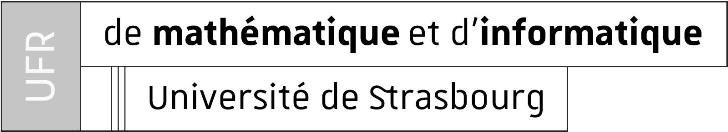
\includegraphics[width = 10cm]{LOGO-UFR-MAI}
\end{center}


\vspace{1cm}
	
{\Large
Internship report
}

\vspace{2cm}

%Titre du mémoire
{\LARGE
{\bf The Riemann-Hilbert correspondence}
}

%Le cas échéant, vous pouvez inclure sur la page de garde une image significative tirée du mémoire

\vspace{10cm}

%votre prénom et nom
{\Large 
by 

Damien \textsc{Junger}
}

\vspace{1cm}
%nom de l'encadrant ou encadrante
{\Large 
supervised by

Annette \textsc{Huber-Klawitter}
}

\vfill
%Année
{\Large 
2026	
}


\end{center}	

\pagebreak

\thispagestyle{empty}

\qquad 


\setcounter{page}{0}

\vfill\pagebreak 


\vspace*{0.03\textheight}

%\hspace{1 cm} Je souhaite remercier

\vspace*{0.5\textheight}

%\begin{flushright}
%\textit{« Là-haut, la terre est bleue comme une orange »} \\
%Livre ancien, \textit{Mur de la tour d'Ær}
%\end{flushright}

\pagebreak


%%%%%%%%%%%ù


\tableofcontents
\newpage



\section{Prerequisites}


\subsection{Category theory}

\begin{mydef}
A \textit{category} $\cat{C}$ is given by the data of :
\begin{itemize}
\item[1.] a class Ob$(\cat{C})$, called the \textit{class of objects} of $\cat{C}$,
\item[2.] for every couple of objects $(x,y)$ of $\cat{C}$, a class $\Hom_\cat{C}(x,y)$, called the \textit{class of morphisms} from $x$ to $y$,
\item[3.] for every triplet of objects $(x,y,z)$ of $\cat{C}$, a function 
\begin{center}
	$\fonction{\text{comp}_{(x,y,z)}}{\Hom_\cat{C}(x,y) \times \Hom_\cat{C}(y,z)}{\Hom_\cat{C}(x,z)}{(f,g)}{g\circ f}$
\end{center}
satisfying the following proprerties :
\begin{itemize}
\item[a.] (\textit{Associative law}) for every quartet of objects $(w,x,y,z)$ of $\cat{C}$, if $(f,g,h)\in \Hom_\cat{C}(w,x) \times \Hom_\cat{C}(x,y) \times \Hom_\cat{C}(y,z)$, then $(h\circ g)\circ f = h\circ (g\circ f)$,
\item[b.] (\textit{Identities}) for every object $x$ of $\cat{C}$, there exists an element $1_x$ of $\Hom_\cat{C}(x,x)$, so that for every couple of objects $(w,y)$ and every morphisms $(f,g)\in \Hom_\cat{C}(w,x)\times \Hom_\cat{C}(x,y)$, then $1_x\circ f = f$ and $g\circ 1_x = g$.\\

\end{itemize}
$g \circ f$ is called the \textit{composition} of $g$ with $f$.
\end{itemize}

\end{mydef}


\begin{myrem}
\begin{itemize}
\item[1.] We will use the following notations : $x\in \text{Ob}(\cat{C})$ if $x$ in an object of $\cat{C}$, $f: x\to y$ if $f$ is an element of $\Hom_\cat{C}(x,y)$.
\item[2.] If $f:x\to y$, $x$ is called the \textit{domain} or \textit{source} of $f$ and $y$ the \textit{codomain} or \textit{target} of $f$.
\item[3.] For our purpose, it is sufficient to consider that for every $(x,y)\in \text{Ob}(\cat{C})^2$, $\Hom_\cat{C}(x,y)$ is a set. In this case, the category is said to be \textit{locally small}.
\end{itemize}
\end{myrem}

\begin{mydef}
Let $\cat{C}$ be a category.\\
A category $\cat{D}$ is said to be a \textit{subcategory} of $\cat{C}$ if the following are satisfied :
\begin{itemize}
\item[1.] every object of $\cat{D}$ is an object of $\cat{C}$,
\item[2.] for every $(x,y)\in \text{Ob}(\cat{D})^2$, then $\Hom_\cat{D}(x,y) \subseteq \Hom_\cat{C}(x,y)$,
\item[3.] for every $x\in\text{Ob}(\cat{D})$, then $1_x \in \Hom_\cat{D}(x,x)$,
\item[4.] for every $(x,y,z)\in\text{Ob}(\cat{D})^3$, every $(f,g)\in\Hom_\cat{D}(x,y)\times \Hom_\cat{D}(y,z)$, then $g\circ f \in \Hom_\cat{D}(x,z)$.
\end{itemize}
$\cat{D}$ is said to be a \textit{full subcategory} of $\cat{C}$ if in addition, for every $(x,y)\in \text{Ob}(\cat{D})^2$, then $\Hom_\cat{D}(x,y) = \Hom_\cat{C}(x,y)$.
\end{mydef}





\subsection{Sheaf theory}



In the following, $X$ is a topological space and $\Tau_X$ will denote its topology category. 

\begin{mydef}

Let $\cat{C}$ be a category (often $\cat{C} = \mathscr{Set}, \mathscr{Ab}, \mathscr{Rings}$...).\\
A \textit{presheaf} of $\cat{C}$ is a contravariant functor $\sheaf : \Tau_X \to \cat{C}$.\\
Explicitly, it is the data of :
\begin{itemize}
\item[1.] for every open set $U$ of $X$, an object $\sheaf(U)$ of $\cat{C}$,
\item[2.] for every couple of open sets $V \subseteq U$ of $X$, a morphism $\res_{U,V} : \sheaf(V) \to \sheaf(U)$ verifying :
\begin{itemize}
\item[a.] for every open set $U$ of $X$, then $\res_{U,U} = \text{id}_U$,
\item[b.] for every open sets $U\subseteq V \subseteq W$ of $X$, then $\res_{U,V} \circ \res_{V,W} = \res_{U,W}$.
\end{itemize}
\end{itemize}
The objects $\sheaf(U)$ are often called \textit{sections of $\sheaf$ over $U$}, and for avoiding confusion, will we denoted $\Gamma(U,\sheaf)$.
\end{mydef}

\begin{myrem}
If the context is clear, we will denote $\text{res}_{U,V}(f) = f|_U$ (the notation is justified in the next lines).
\end{myrem}

\begin{myex}
\begin{itemize}
\item[1)] The sheaf of real valued continuous functions $C^0(\--,\RR)$ with classical restriction functions $\res(U,V)(f) = f|_U$.
\item[2)] If $X$ has an additional structure, the above example can be further specified : if $X$ is a differentiable manifold, we can consider $C^\infty(\--,\RR)$, if $X$ is a complex manifold, $\holo(\--,\CC)$ ...
\item[3)] If $C$ is an object of $\cat{C}$, the constant presheaf $\underline{C}$. We will be intersted in $\underline{\ZZ}$ or $\underline{\CC}$.
\item[4)] The sheaf of real valued bounded functions $B(\--,\RR)$.
\end{itemize}
\end{myex}

Presheaves comes from a category point of view, so we need morphisms :

\begin{mydef}
A \textit{morphism of presheaves} (over the same space $X$) $\varphi : \sheaf \to \mathcal{G}$ is a natural transformation.\\
More explicitly, it is the data, for each $U\in \Tau_X$, of a morphism $\varphi_U : \sheaf(U) \to \mathcal{G}(U)$ of $\cat{C}$ such that the following diagram commutes for every $U \subseteq V$ :
\begin{center}
\begin{tikzcd}
\sheaf(V) \arrow[r, "\varphi_V"] \arrow[d, "\res^{\sheaf}_{U,V}" left]
& \mathcal{G}(V) \ \arrow[d, "\res^{\mathcal{G}}_{U,V}"] \\
\sheaf(U) \arrow[r, "\varphi_U"]
& \mathcal{G}(U)
\end{tikzcd}
\end{center}
\end{mydef}


\begin{mydef}
A \textit{sheaf} $\sheaf$ is a presheaf satisfying the extra conditions for any open cover $\{U_i,i\in I\}$ of an open set $U$ of $X$:
\begin{itemize}
\item[3.] for every $f,g \in \sheaf(U)$ such that : $\forall i \in I,~ f|_{U_i} = g|_{U_i}$, then $f = g$.
\item[4.] for every $(f_i)\in \prod_{i\in I} \sheaf(U_i)$ such that : $\forall (i,j)\in I^2,~ f_i|_{U_i \cap U_j}= f_j|_{U_i \cap U_j}$, then there exists $f\in\sheaf(U)$ with $f|_{U_i} = f_i$ for any $i\in I$.
\end{itemize}
\end{mydef}


\begin{myrem}
For $U = \emptyset$, it says that $\sheaf(\emptyset)$ is the terminal object of $\cat{C}$ (if such one exists). Indeed, we can take the open covering of $\emptyset$ by a family indexed by $\emptyset$ itself, and we then have an arrow $\sheaf(\emptyset) \to $
\end{myrem}

\begin{myex}
\begin{itemize}
\item 1) and 2) are indeed sheaves.
\item 3) is not, because of the previous remark.
\item 4) is not either, with the conter example $\RR = \bigcup_{n\in \NN} ~(-n,n)$ and $f : x\mapsto x$.
\item If $X$ is Hausdorff, $x_*$ is a point of $X$, $(S,s)$ a pointed set, the \textit{skycraper sheaf} is given by $\sky_{x_*}(S) : U \mapsto \left\lbrace
\begin{array}{l l}
S & \text{if } x_* \in U \\
s & \text{otherwise}.
\end{array}
\right.
$
\end{itemize}
\end{myex}

\begin{mydef}
We will denote by $\text{PSh}_X$, respectively $\text{Sh}_X$, the category of presheaves, respectively the full subcategory of sheaves, over $X$.
\end{mydef}

One can ask what looks like the behavior of the sheaf very locally, on a point. Since a singleton is in general not a point, we need the following definition.

\begin{mydef}
Let $\sheaf$ be a (pre)sheaf.\\
We define the \textit{stalk} at $x\in X$ as :
\begin{center}
$\sheaf_x := \quot{\{(U,s) | ~x\in U, ~U \in \Tau_X, ~s \in \sheaf(U)\}}{\sim}~,$
\end{center}
where $(U,s) \sim (V,t) \Leftrightarrow (\exists W \subset U \cap V): s|_W = t|_W$.
\end{mydef}

\begin{myrem}
From a categorical point of view, it is also the direct limit : $\sheaf_x = \underset{\overrightarrow{U \ni x}}{\lim} \sheaf(U)$, where the limit is taken over open set $U$.
\end{myrem}

It turns out that this localization principle can be used to transform a presheaf into a sheaf in a natural way (in the sense of what follows).

\begin{mydef}
Let $\sheaf$ be a presheaf.\\
We define for every open set $U$
\begin{center}
$\d \sheaf^{\sharp}(U) = \left\lbrace s : U \to \coprod_{x\in U} \sheaf_x ~\left|\right.~ \left\lbrace 
\begin{array}{l}
\forall x\in U,~ s(x) \in \sheaf_x\\
\exists V \subset U,\exists t\in \sheaf(V) \text{ s.th.} \forall y\in V,~ s(y) = t(y)
\end{array}
\right. \right\rbrace$.
\end{center}
$\sheaf^\sharp$ is called the \textit{sheafification of $\sheaf$}.
\end{mydef}

\begin{myprop}
$\sheaf^\sharp$ is a sheaf.
\end{myprop}

\begin{myex}
$\underline{\RR}^\sharp$ is the sheaf of locally constant functions, more precisely the sheaf of continuous functions $C^0(\--,\RR)$, where $\RR$ is equipped with the discrete topology.
\end{myex}



\begin{myprop}
$((\--)^\sharp,\text{Forget})$ is an adjoint pair of functors between $\text{PSh}_X$ and $\text{Sh}_X$.
\end{myprop}

\begin{mydemo}
.
\end{mydemo}

\begin{myex}
Suppose that $\cat{C}$ admits kernels and cokernels (this assumption holds whenever kernels and cokernels are written). \\
For $\varphi: \sheaf \to \mathcal{G}$, we define $\Ker(\varphi)(U) := \Ker(\varphi_U)$, $\text{Im}(\varphi)(U) := \text{Im}(\varphi_U)$ and $\text{Coker}(\varphi)(U) := \text{Coker}(\varphi_U)$.\\
The first one is always a sheaf, but the two others are not in general. In the following, $\text{Im}(\varphi)$ or $\text{Coker}(\varphi)$ will always denote the sheafification of these presheaves.
\end{myex}

\begin{myprop}
A complex $0 \to \sheaf \to \mathcal{G} \to \mathcal{H} \to 0$ is exact if, and only if the induced complex on stalks $0 \to \sheaf_x \to \mathcal{G}_x \to \mathcal{H}_x \to 0$ is exact for every $x\in X$.
\end{myprop}

\begin{mydemo}
.
\end{mydemo}

\begin{myrem}
In general, it is not equivalent of the exactness of the induced sequence over every open set $U$.\\
One could take as a counterexample the exponential sequence on $\CC$ :
\begin{center}
$
\begin{array}{c c c c c c c c c}
0 & \to & \underline{\ZZ} & \to & \holo_\CC & \to & \holo_\CC^* & \to & 0,\\
  &     &                &     &   f       & \mapsto & \exp(2\pi i f) & &\\
\end{array}
$
\end{center}
that is not exact over $\CC^*$, because the map $\holo_{\CC^*} \to \holo_{\CC^*}^*$ is not surjective : the map $z \mapsto z$ does not belong to the image since $\log$ is not well defined over $\CC^*$.
\end{myrem}


\begin{myprop} \label{patching_sheaf}
Let $X = \cup_{i\in I} U_i$ an open covering of $X$. For every $i\in I$, let $\sheaf_i$ a sheaf on $U_i$.\\
Assume that for every $i \neq j \in I$, there exists an isomorphism 
\begin{center}
$\theta_{i,j} : \sheaf_i|_{U_i \cap U_j} \overset{\sim}{\to} \sheaf_j|_{U_i \cap U_j}$,
\end{center}
satisfying the condition $\theta_{j,k} \circ \theta _{i,j} = \theta_{i,k}$ on $U_i \cap U_j \cap U_k$ for every triplet of distinct elements of $I$.\\
Then, there exists a sheaf $\sheaf$ on $X$ such that for every $i\in I, \sheaf|_{U_i} = \sheaf_i$. Moreover, this sheaf is unique, up to unique isomorphism.
\end{myprop}

\begin{mydemo}
.
\end{mydemo}

\subsection{Complex geometry}

\subsubsection{First definitions}

\begin{mydef}
Let $X$ be a differentiable manifold of dimension $2n$.\\
An \textit{holomorphic atlas} is a set $\{(U_i,\varphi_i),i\in I\}$ where $X = \bigcup_{i\in I} U_i$ is an open cover and $\varphi : U_i \to \CC^n$ are homeomorphism on their image, such that for all $(i,j)\in I^2$, the \textit{transition map} $\varphi_j \circ \varphi_i^{-1} : \varphi_i(U_i \cap U_j) \to \varphi_j(U_i \cap U_j)$ is holomorphic. 

\smallskip
Such a couple $(U_i,\varphi_i)$ is called a \textit{local coordinate system}, or just \textit{coordinates}.

\smallskip
We say that two holomorpic atlases $\{(U_i,\varphi_i),i\in I\}$ and $\{(\tilde{U_j},\tilde{\varphi_j}),j\in J\}$ are \textit{equivalent} if for all $(i,j)\in I\times J, \tilde{\varphi_j} \circ \varphi_i^{-1} : \varphi_i(U_i \cap \tilde{U_j}) \to \tilde{\varphi_j}(U_i \cap \tilde{U_j})$.
\end{mydef}

\begin{mydef}
A \textit{complex manifold of dimension $n$} is a real manifold $X$ of dimension $2n$ endowed with an equivalence class of holomorphic atlases. 
\end{mydef}

\begin{myrem}
In the following, unless explicitly stated otherwise, the complex manifold will be endowed with an representant of the equivalente class, denoted by $\{(U_i,\varphi_i),i\in I\}$.
\end{myrem}

\begin{mydef}
Let $X$ be a complex manifold and $f : X \to \CC$.\\
We say that $f$ is \textit{holomorphic} if for all local coordinates $(U,\varphi), f\circ \varphi : \varphi(U) \to \CC$ is holomorphic.
\end{mydef}

\begin{mydef}
Let $X$ be a complex manifold.\\
We denote by $\holo_X$ the sheaf of holomorphic function on $X$, \textit{ie} $\holo_X : U \mapsto \{f:U \to \CC, f\text{ holomorphic}\}$.
\end{mydef}

\begin{myrem}
$\holo_{X,x}$ will denote the stalk of $\holo_X$ at $x$. It coincides with the germs of holomorphic functions at $x$. \textit{Via} local coordinates $(U,\varphi)$, with $\varphi(x_*)=0$ for some $x_*\in U$, we have an isomorphism $\holo_{X,x} \simeq \holo_{\CC^n,0}$. It is an integral domain, and we denote by $Q(\holo_{X,x})$ the quotient field associated.
\end{myrem}

More generally, if the codomain is also a complex manifold, we have the following definition :

\begin{mydef}
Let $X$ and $Y$ be complex manifolds and $f : X \to Y$ continuous.\\
We say that $f$ is \textit{holomorphic} if for all local coordinates $(U,\varphi)$ on $X$ and $(U',\varphi')$ on $Y$, $\varphi'\circ f\circ \varphi : \varphi(U \cap f^{-1}(U')) \to \varphi'(U')$ is holomorphic.
\end{mydef}

\begin{mydef}
Let $X$ be a complex manifold.\\
A \textit{meromorphic function} on $X$ is a map $f : X \to \bigsqcup_{x\in X} Q(\holo_{X,x})$ so that, for all $x_* \in X$, there exists an open neighborhood $U \subset X$ of $x_*$ and $g,h \in \holo_U$ verifying : $(\forall x\in U), ~f_x = \frac{g}{h}$.

\smallskip
The sheaf of meromorphic functions is denoted $\mero_X$.
\end{mydef}

\begin{myrem}
If $U\subset X$ is an connected open subset, then $\mero_X(U)$ is a field, and if $X$ itself is connected, $\mero(X) = \mero_X(X)$ is called the function field of $X$.
\end{myrem}


\subsubsection{Vector bundle}

\begin{mydef}
Let $X$ be a complex manifold and $r$ a positive integer.\\
A \textit{holomorphic vector bundle} or rank $r$ on $X$ is a complex manifold $E$ equipped with a holomorphic map $\pi : E \to X$ such that :
\begin{itemize}
\item[1.] for all $p \in X$, the \textit{fiber} $E_p := \pi^{-1}(p)$ is a complex vector space of dimension $r$,
\item[2.] there exists an open covering $X = \bigcup_{i\in I} U_i$ and biholomorphic maps $\psi_i : \pi^{-1}(U_i) \to U_i \times \CC^r$, called the \textit{trivialization maps}, satisfying :
\begin{itemize}
\item[a.] the following diagram commutes :
\begin{center}

\begin{tikzcd}[column sep=small]
\pi^{-1}(U_i) \arrow[rr, "\psi_i"] \arrow[dr, "\pi"] & & U_i \times \CC^r \arrow[dl,"\text{pr}_1"]\\
& U_i &
\end{tikzcd}

\end{center}
\item[b.] The induced map $E_p \to \CC^r$ for any $p\in U_i$ is $\CC$-linear.
\end{itemize}
\end{itemize}

\smallskip
If $r=1$, we say that $(E,\pi)$ is a \textit{line bundle}.
\end{mydef}

\begin{myrem}
The travialization maps induce linear isomorphisms $\psi_{i,j} = \psi_i \circ \psi_j^{-1} :U_i \cap U_j \to \GL_r(\CC)$, and the collection $\{\psi_{i,j},i,j\in I\}$ is called a cocycle.\\
In particular, it verifies the conditions :
\begin{itemize}
\item[i.] $\psi_{i,i} = \text{id}_{U_i}$,
\item[ii.] $\psi_{j,k}\circ \psi_{i,j} = \psi_{i,k}$.
\end{itemize}
\end{myrem}


\begin{myprop}
Let $X$ be a complex manifold and let $r$ be a positive integer.\\
The categories $\vectbun^r(X)$ and $\locfree_r(X)$ are equivalent.
\end{myprop}

\begin{mydemo}
We define 
\begin{center}
$\fonction{\sheaf}{\vectbun_r(X)}{\locfree_r(X)}{E}{\sheaf_E}$,
\end{center}
where $\sheaf_E$ is the sheaf of sections of $E$. It is well defined by ??.\\
It is a functor : given a morphism of vector bundles $f:E_1 \to E_2$, we define for each open set $U$ of $X$ the function
\begin{center}
$\fonction{\varphi_U}{\sheaf_1(U)}{\sheaf_2(U)}{s}{f\circ s}$.
\end{center}
$\varphi$ clearly defines a morphism of sheaves.\\
In order to construct a quasi-inverse, let $\sheaf \in \mathcal{S}_X$ and $\psi : \sheaf(U_i) \to \holo_{U_i}{\vphantom{\holo}}^{\oplus r}$ local trivialisations on an open cover $\{U_i,i \in I\}$ of $X$.
\end{mydemo}


\subsubsection{Connections}

\begin{mydef}
Let $\erond$ be a locally free $\holo_X$-modules.\\
A \textit{connection on $\erond$} is a $\CC$-linear application $\nabla : \erond \to \erond \otimes_{\holo_X} \Omega_X^1$ satisfying the \textit{Liebniz relation} : for any local sections $s$ and local function $f$, then
\begin{center}
$\nabla(fs) = df \otimes s + f\nabla(s)$.
\end{center}
In particular, it induces, for each integer $k >0$, a $\CC$-linear map
\begin{center}
$\fonction{\nabla^{(k)}}{\erond \otimes_{\holo_X} \Omega_X^k}{\erond \otimes_{\holo_X} \Omega_X^{k+1}}{s \otimes \omega}{(-1)^k\nabla s \wedge \omega + s \otimes dw}$
\end{center}
A connection $\nabla$ is said to be \textit{flat} (or \textit{integrable}) if the \textit{curvature} $K := \nabla^{(1)} \circ \nabla$ is zero.
\end{mydef}

\begin{myrem}
In dimension 1, we have $\Omega_X^2 = 0$, so all connections are flat.
\end{myrem}

\begin{myex}
\begin{itemize}
\item[1)] $d$ is a connection on $\holo_X$ by identifying $\holo_X \tensor{\holo_X} \Omega_X^1 \simeq \Omega_X^1$. It induces a connection on $\holo_X^r$ acting coordinate-wise.
\item[2)] For every $\omega \in\Omega_X^1$, the map
\begin{center}
$\fonction{d+\omega}{\holo_X}{\Omega_X^1}{f}{df +\omega f}$
\end{center}
is a connection. More generally, if $\omega$ is a $r \times r$ matrix with coefficients in $\Omega_X^1$, the map $d + \omega$ is a connection on $\holo_X^r$.
\end{itemize}
\end{myex}

The following result says that these are the only ones on $\holo_X^r$, and then the only ones locally on $\erond$.

\begin{mylemme}
Every connection $\nabla$ on $\holo_X^r$ is written $d + \omega$ for some $\omega$ as above.
\end{mylemme}

\begin{mydemo}
For every $f \in \holo_X$ and $h \in \holo_X^r$, we have by the Liebniz rule :
\begin{center}
$(\nabla - d)(fh) = f\nabla(h) + df \otimes h - fdh - df \otimes h = f(\nabla - d)h$.
\end{center}
Thus, $\nabla - d : \holo_X^r \to \Omega_X^1$ is $\holo_X$-linear and it's the multiplication by a matrix $\omega$.
\end{mydemo}

\begin{myrem} \label{connections_diff_eq}
Connections are a reformulation of (systems) of differential equations, locally on a vector bundle.\\
Let $\nabla = d + \omega$ a connection on $\holo_X^r$ (it is of this form by the previous lemma). We choose local coordinates $z^1,\dots,z^n$ on $X$. Then we can write 
\begin{center}
$\d \omega(z) = \sum_{j=1}^n A_i(z) dz^j$.
\end{center}
For a $f$ holomorphic on the chart, we then have :
\begin{center}
$\d \nabla f = \sum_{j=1}^n \left(\frac{\partial f}{\partial x^j} + A_j f\right)dz^j$,
\end{center}
and $\nabla f = 0$ is equivalent to :
\begin{center}
$\left\lbrace
\begin{array}{c}
\d \frac{\partial f}{\partial z^1}(z) = A_1(z) f(z),\\
\d \vdots \\
\d\frac{\partial f}{\partial z^n}(z) = A_n(z) f(z),
\end{array}
\right.$
\end{center}
which is a system of \textit{partial} differential equations.\\
\end{myrem}

\begin{mydef}
We define the category $\locfreenabla(X)$ with 
\begin{itemize}
\item locally free $\holo_X$-modules equipped with flat connections as objects,
\item morphisms of $\holo_X$-modules $\varphi : \erond_1 \to \erond_2$ making 
\begin{center}
\begin{tikzcd}
\erond_1 \arrow[r, "\nabla_1"] \arrow[d, "\varphi"]
& \erond_1 \otimes_{\holo_X} \Omega_X^1 \ \arrow[d, "\varphi \otimes 1"] \\
\erond_2 \arrow[r, "\nabla_2"]
& \erond_2 \otimes_{\holo_X} \Omega_X^1
\end{tikzcd}
\end{center}
commutes, as morphisms between $(\erond_1,\nabla_1)$ and $(\erond_2,\nabla_2)$.
\end{itemize}
\end{mydef}

Here are some algebraic construction one can obtain with connections :

\begin{myprop} \label{algebraic_construction_connection}
Let $(\erond_1,\nabla_1)$ and $(\erond_2,\nabla_2)$ two connections on $X$. The followings are also connections :
\begin{itemize}
\item[1)] $(\erond_1^*,(\-- \otimes 1)\circ \nabla_1)$, 
\item[2)] $(\erond_1 \oplus \erond_2, \nabla_1 \oplus \nabla_2)$,
\item[3)] $(\erond_1 \tensor{\holo_X} \erond_2, \nabla_1 \otimes 1 + 1 \otimes \nabla_2)$
\item[4)] $(\connHom_{\holo_X}(\erond_1,\erond_2),\phi \mapsto (\nabla_2 \circ \phi) - (\phi \otimes 1) \circ \nabla_1)$
\end{itemize}
\end{myprop}


\section{The Riemann-Hilbert correspondence}

\subsection{A correspondence in algebraic topology}

truc truc


\subsection{Holomorphic version on a complex manifold}



\begin{mytheo}[Riemann-Hilbert correspondence, complex manifold case]
The fonctor
\begin{center}
$\fonction{F}{\locfreenabla(X)}{\locsys(X)}{(\erond,\nabla)}{\erond^{\nabla} := \Ker(\nabla)}$
\end{center}
induces an equivalence of categories.\\
It's inverse is given by
\begin{center}
$\fonction{G}{\locsys(X)}{\locfreenabla(X)}{\arond}{(\holo_X \tensor{\CC} \arond,d\otimes 1)}$
\end{center}
\end{mytheo}

\begin{mydemo}
\begin{itemize}

\item[] \underline{Step 1} :  $G$ is well defined, that is : if $\arond \in \locsys(X)$, then $(\erond,\nabla) := (\arond \tensor{\CC} \holo_X,1\otimes d) \in \locfree^\nabla(X)$.

\smallskip
First remark that $d\otimes 1$ is well defined by extension of $\holo_X \to \Omega^1_X$ with the tensor product. We also use the identification 
\begin{center}
$(\arond \tensor{\CC} \holo_X)\tensor{\holo_X} \Omega^1_X \simeq \arond \tensor{\CC} (\holo_X \tensor{\holo_X} \Omega^1_X) \simeq \arond \tensor{\CC} \Omega^1_X$
\end{center} by super-commutativity of the tensor product.\\
For a small open set such that $\arond|_U \simeq \CC^r$, we have $(\arond \otimes \holo_X)|_U \simeq \arond|_U \otimes \holo_U \simeq \CC^r \otimes \holo_U \simeq \holo_U^{\oplus r}$.\\
Finally, we have :
\begin{center}
$\nabla^{(1)} \circ \nabla (a\otimes f) = \nabla^{(1)} ((a \otimes 1) \otimes df) = \nabla(a \otimes 1) \wedge df + a \otimes d(df) = (a \otimes d1) \wedge df = 0$.
\end{center}
We again used that the image of $a \otimes f$ in $\erond \tensor{\holo_X} \Omega^1_X$ is identified with $(a \otimes 1) \otimes df$.


\item[] \underline{Step 2} : $G$ is a functor.

\smallskip
If $\phi : A \to B$ is a morphism in $\locsys(X)$, we have an induced $G(\phi) = \phi \otimes 1 : A \tensor{\CC} \holo_X \to B \tensor{\CC} \holo_X$ that makes the following commutes :
\begin{center}
\begin{tikzcd}
A \tensor{\CC} \holo_X \arrow[r, "\phi \tensor 1"] \arrow[d, "1 \otimes d" left]
& A \tensor{\CC} \holo_X \ \arrow[d, "1 \otimes d"] \\
A \tensor{\CC} \Omega^1_X \arrow[r, "\phi \otimes 1"]
& B \tensor{\CC} \Omega^1_X
\end{tikzcd}
\end{center}


\item[] \underline{Step 3} : $F$ is well defined, that is : if $(\erond,\nabla) \in \locfree(X)$, then $\erond^\nabla \in \locsys(X)$.

\smallskip
This is the most difficult part. Let's sketch out the proof.\\
The result is equivalent to saying that \textit{locally}, the solutions of our system of differential equations given by $\nabla$ is a complex vector space, with dimension equal to the rank of the system. One can then think of the Cauchy-Lipschitz theorem.


\item[] \underline{Step 4} : $F$ is a functor.

\smallskip
If $\phi : (\erond_1,\nabla_1) \to (\erond_2,\nabla_2)$ a morphism in $\locfree^\nabla(X)$, then it induces a morphism of sheaves $\phi : \Ker(\nabla_1) \to \erond_2$, and its image is a subset of $\Ker(\nabla_2)$ by the relation $\nabla_2 \circ \phi = (f\otimes 1)\circ \nabla_1$.


\item[] \underline{Step 5} : $GF \simeq 1_{\locfree^\nabla(X)}$.

\smallskip
Let $(\erond,\nabla) \in \locfree^\nabla(X)$. Set
\begin{center}
$\fonction{\alpha_{(\erond,\nabla)}}{\Ker(\nabla) \tensor{\CC} \holo_X}{\erond}{s \otimes f}{fs}$.
\end{center}
It is clearly well defined and for $s \otimes f \in \Ker(\nabla) \tensor{\CC} \holo_X$, we have :
\begin{center}
$\nabla(\alpha(s \otimes f))=\nabla(fs) = s \otimes df = \alpha(s \otimes 1)\otimes df = (\alpha\otimes 1)((1 \otimes d)(s \otimes f))$,
\end{center}
so $\varphi$ define a morphism in the category $\locfree^\nabla(X)$.\\
Better, it defines a natural transformation. Let $\phi :(\erond_1,\nabla_1)\to(\erond_2,\nabla_2)$ a morphism in $\locfree^\nabla(X)$. Then,
\begin{center}
$\phi(\alpha_{(\erond_1,\nabla_1)}(f\otimes s)) = \phi(fs)$
\end{center}
and
\begin{center}
$\alpha_{(\erond_2,\nabla_2)}(GF(\phi)) = \alpha_{(\erond_2,\nabla_2)}(F(\phi)(s)\otimes f) = f\phi(s)$.
\end{center}
This is equal because $\phi$ is a morphism of $\holo_X$-modules.\\
We define an inverse $\beta_{(\erond,\nabla)}$ locally. For an open set $U$ such that $\erond_U \simeq \holo_U^{\oplus r}$, we set $(s_1, \dots, s_r)$ a basis of $\erond(U)$. Then a section $\sigma \in \erond(U)$ is uniquely written as $\sigma = \sum_{i=1}^r f_i s_i$, and we define $\beta_{(\erond,\nabla)}(\sigma) = \sum_{i = 1}^r f_i \otimes s_i$. It clearly does not depend on the basis, since two basis differ from one another by a matrix with constant coefficients, and therefore	 commutes with the tensor product.\\
Still localy, we have $\alpha_{(\erond,\nabla)} \circ \beta_{(\erond,\nabla)} = $


\item[] \underline{Step 6} : $FG \simeq 1_{\locsys(X)}$.

\smallskip
We clearly have for a local system $\arond$ on $X$, $(\arond \tensor{\CC} \holo_X)^{1 \otimes d} \simeq \arond \tensor{\CC} \CC \simeq \arond$, and it behaves well with morphisms, such that it defines an isomorphism of functors.



\end{itemize}
\end{mydemo}

\subsection{Meromorphic version on a complex manifold}

\subsubsection{In dimension 1}
\subsubsection{Sketch of a proof in higher dimension}

blabla \cite{huybrechts_complex_geo}
\section{Periods}

for introduction : picard fuschs equation : from periods depending of a parameter, construct a differential equations attached



\nocite{*}
\printbibliography


\end{document}